 %%Définir le format du document: papier, taille de police, type de document, etc.

\documentclass[11pt, English]{article}

%%%%%%%%%% Packages externes utilisés %%%%%%%%%%%%%%%%%%%
\usepackage[English]{babel}
\selectlanguage{english}
\usepackage[T1]{fontenc}
\usepackage[utf8]{inputenc}

\usepackage{verbatim}
\usepackage{graphicx}
\usepackage{epstopdf}
\usepackage{algorithm}
\usepackage{algorithmic}
%\usepackage{algorithm2e}


%La mise en page du rapport, NE PAS MODIFIER.
\usepackage{geometry}
 \geometry{
 a4paper,
 left=20mm,
 right=20mm,
 top=20mm,
 bottom=20mm,
 }

%%%%%%%%% Le corps du document entre begin et end %%%%%%%%%%%%%%%%%%%
\begin{document}

%Page de garde
%%%%%%%%%%%%%%% Page de garde %%%%%%%%%%%%%%%%%%%

\begin{titlepage}{
    \begin{center}
        \vspace* {25mm}
        {\Large \textbf {Université of Cergy-Pontoise}} \\
        \vspace* {10mm}
        {\Large \textbf {REPORT}} \\
        \vspace* {10mm}
        for the Project developing application for mobile devices\\
        \textbf {Licence of Computer Science third year} \\
        \vspace* {10mm}
        	on the subject \\
        \vspace* {10mm}
	{\Huge \textsf{TITRE APPLI}} \\
        \vspace* {10mm}
 	written by \\
        \vspace* {10mm}
        {\Large \textbf {GOUGEROT Elisa \& \& }} \\
            \vspace* {5mm}
        {\Large \textbf {}} \\
				\vspace* {10mm}
        	\begin{figure}[h]
        	    \centering 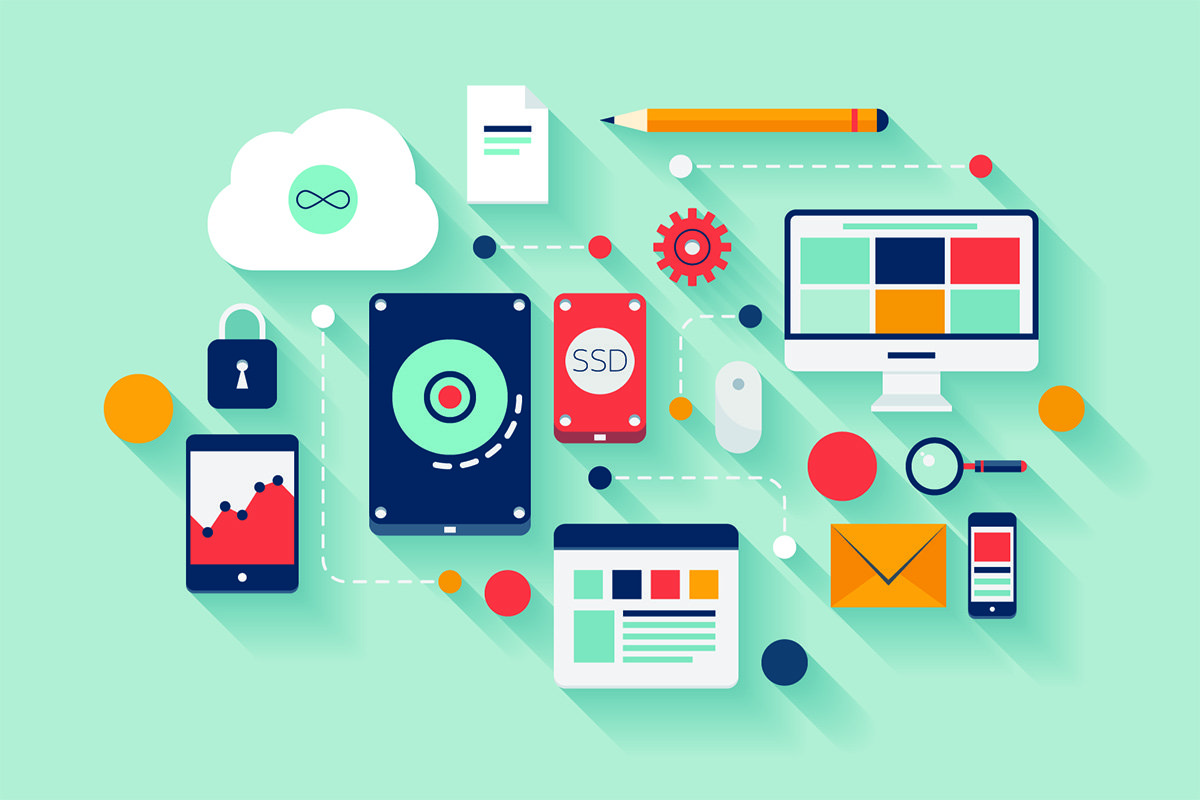
\includegraphics[width=10cm, height=7cm]{images/intro.jpg}
        	    \label{fig:logo}
        	\end{figure}
        \date{} January 2019
        \vspace* {10mm}
	\end{center}
}
\end{titlepage}

%Génération automatique de la table des matières, de la liste des figures et de la liste des tableaux
\tableofcontents
\listoffigures



\newpage
\section{Introduction}
\label{sec:introduction}
\newpage


\section{Specification}
\label{sec:specification}

\newpage
\section{Production}
\label{sec:realisation}
\newpage
\section{Manuel utilisateur}
\label{sec:manuel}
\newpage
\section{Progress of the project}
\label{sec:deroulement}
\newpage
\section{Conclusion}
\label{sec:conclusion}

\subsection{Identified issues and solutions} 

\subsection{Possible improvements}

\end{document}
